\documentclass[10pt, a4paper]{article}

%%% SST LAB PROTOCOLL PREAMBLE
%%% 2019
%%%%%%%%%%%%%%%%%%%%%%%%%%%%%%%


%%% PACKAGES
%%%%%%%%%%%%%%%%%%%%%%%%%%%

\usepackage[ngerman]{babel}

\usepackage[utf8]{inputenc}
\usepackage{amsmath}
\usepackage{pgfplots}
\usepackage{tikz}
\usepackage[many]{tcolorbox}
\usepackage{graphicx}
\graphicspath{ {./graphics/} }
\usepackage{pdfpages}
\usepackage{dashrule}
\usepackage{float}
\usepackage{siunitx}
\usepackage{trfsigns}
\usepackage{booktabs}
\usepackage[european]{circuitikz}
\usepackage{tcolorbox}

%%% DOCUMENT GEOMETRY
%%%%%%%%%%%%%%%%%%%%%%%%%%%

\usepackage{geometry}
\geometry{
 a4paper,
 total={0.6180339887498948\paperwidth,0.6180339887498948\paperheight},
 top = 0.1458980337503154\paperheight,
 bottom = 0.1458980337503154\paperheight
 }
\setlength{\jot}{0.013155617496424828\paperheight}
\linespread{1.1458980337503154}

\setlength{\parskip}{0.013155617496424828\paperheight} % paragraph spacing


%%% COLORS
%%%%%%%%%%%%%%%%%%%%%%%%%%%

\definecolor{red1}{HTML}{f38181}
\definecolor{yellow1}{HTML}{fce38a}
\definecolor{green1}{HTML}{95e1d3}
\definecolor{blue1}{HTML}{66bfbf}
\definecolor{hsblue}{HTML}{00b1db}
\definecolor{hsgrey}{HTML}{afafaf}

%%% CONSTANTS
%%%%%%%%%%%%%%%%%%%%%%%%%%%
\newlength{\smallvert}
\setlength{\smallvert}{0.0131556\paperheight}


%%% COMMANDS
%%%%%%%%%%%%%%%%%%%%%%%%%%%

% differential d
\newcommand*\dif{\mathop{}\!\mathrm{d}}

% horizontal line
\newcommand{\holine}[1]{
  	\begin{center}
	  	\noindent{\color{hsgrey}\hdashrule[0ex]{#1}{1pt}{3mm}}\\%[0.0131556\paperheight]
  	\end{center}
}

% mini section
\newcommand{\minisec}[1]{ \noindent\underline{\textit {#1} } \\}

% quick function plot
\newcommand{\plotfun}[3]{
  \vspace{0.021286\paperheight}
  \begin{center}
    \begin{tikzpicture}
      \begin{axis}[
        axis x line=center,
        axis y line=center,
        ]
        \addplot[draw=red1][domain=#2:#3]{#1};
      \end{axis}
    \end{tikzpicture}
  \end{center}
}

% box for notes
\newcommand{\notebox}[1]{

\tcbset{colback=white,colframe=green1!100!black,title=Note!,width=0.618\paperwidth,arc=0pt}

 \begin{center}
  \begin{tcolorbox}[]
   #1 
  \end{tcolorbox}
 
 \end{center} 
 
}

% box for equation
\newcommand{\eqbox}[2]{
	
	\tcbset{colback=white,colframe=green1!100!black,title=,width=#2,arc=0pt}
	
	\begin{center}
		\begin{tcolorbox}[ams align*]
				#1
		\end{tcolorbox}
		
	\end{center} 
	
}
% END OF PREAMBLE

\addbibresource{sources.bib}
\addbibresource{web.bib}

\begin{document}

%
\includepdf{./titlepage/titlepage.pdf}
%\pagebreak

\begin{center}
  \Large{Einfacher COTS Performance-Benchmark}
\end{center}

\begin{flushright}
  R. Grünert\\
  \today
\end{flushright}

\begin{flushleft}
  CPU: i7 4790k
\end{flushleft}

\section{Erster Benchmark}


\begin{figure}[h]
  \begin{center}
    \inputminted{rust}{./code/main.rs}
  \end{center}
  \caption{Erstes Benchmarkprogramm.}
  \label{fig:progi}
\end{figure}




Für einen ersten Performancetest wurde das in Listing \ref{fig:progi} gezeigte Programm in Rust geschrieben.
Es berechnet lediglich die durch Aufrufargumente übergebene Anzahl an (32-bit-) Fließpunktmultiplikationen (Zeile 22).
In diesem Fall wurde \inlinecodee{num\_iterations=40000000000} gewählt.\\

Das Programm wurde mit zwei unterschiedlichen Optimierungsstufen kompiliert \cite{profiles}:
\begin{itemize}
  \item Sog. \glqq{}release\grqq-Modus (\inlinecodee{opt-level 3})
  \item Keine Optimierung (\inlinecodee{opt-level 0})
\end{itemize}

\begin{table}[H]
  \centering
\begin{tabular}{|l|l|l|}
\hline
opt-level & Zeit / s & Perf. / GFLOPS \\ \hline
0         & $14.529$ & $2.753$        \\ \hline
3         & $4.675$  & $8.557$        \\ \hline
\end{tabular}
\caption{Ergebnisse des ersten Benchmarks.}
\end{table}

\section{Zweiter Benchmark}

\begin{figure}[H]
  \begin{center}
    \inputminted{rust}{./code/main2.rs}
  \end{center}
  \caption{Zweites Benchmarkprogramm.}
  \label{fig:programm3}
\end{figure}

In einem weiteren Test wurde das erste Programm modifiziert, um parallele Vektoroperationen zu testen. Erneut wurde mit zwei Optimierungsstufen kompiliert.\\

Lässt man sich den generierten Assembler-Code dieses Programmes ausgeben\footnote{ \inlinecodee{cargo rustc --release -- --emit asm}}, findet man im Fall der optimierten Kompilierung die Schleife der Zeilen 26 bis 36 wieder (Abb. \ref{fig:programm2}). Man erkennt partielles Loop-Unrolling sowie die SIMD-Operationen \inlinecodee{mulps} und \inlinecodee{addps}, welche die Addition bzw. Multiplikation der 4 Arraywerte in einer einzigen 128-bit Operation ermöglichen (siehe \cite{wiki_sse}). Dies ist natürlich ein konstruiertes Szenario, welches die SIMD-Operationen bevorzugt, was sich auch in der erhöhten Performance wiederspiegelt (Tabelle \ref{fig:simdm}).

\begin{figure}[h]
  \begin{center}
    \inputminted{asm}{./code/simd.s}
  \end{center}
  \caption{Snippet aus dem optimierten Assembler-Code des zweiten Benchmarkprogrammes.}
  \label{fig:programm2}
\end{figure}

\begin{table}[h]
  \centering
\begin{tabular}{|l|l|l|}
\hline
opt-level & Zeit / s & Perf. / GFLOPS \\ \hline
0         & $43.741$ & $7.316$        \\ \hline
3         & $7.867$  & $40.679$        \\ \hline
\end{tabular}
\caption{Ergebnisse des zweiten Benchmarks.}
  \label{fig:simdm}
\end{table}


%\pagebreak

% ------------------------------------------------------------------------------

\printbibheading
%\begin{refsection}[sources.bib]
%\nocite{*}
%\printbibliography[heading=subbibliography,title={Literature}]
%\end{refsection}

\begin{refsection}[web.bib]
\nocite{*}
\printbibliography[heading=subbibliography,title={Web}]
\end{refsection}

%\begin{refsection}[software.bib]
%\nocite{*}
%\printbibliography[heading=subbibliography,title={Software Used}]
%\end{refsection}


%\begin{figure}[H]
    \centering
    \begin{minipage}{0.48\textwidth}
        \centering
        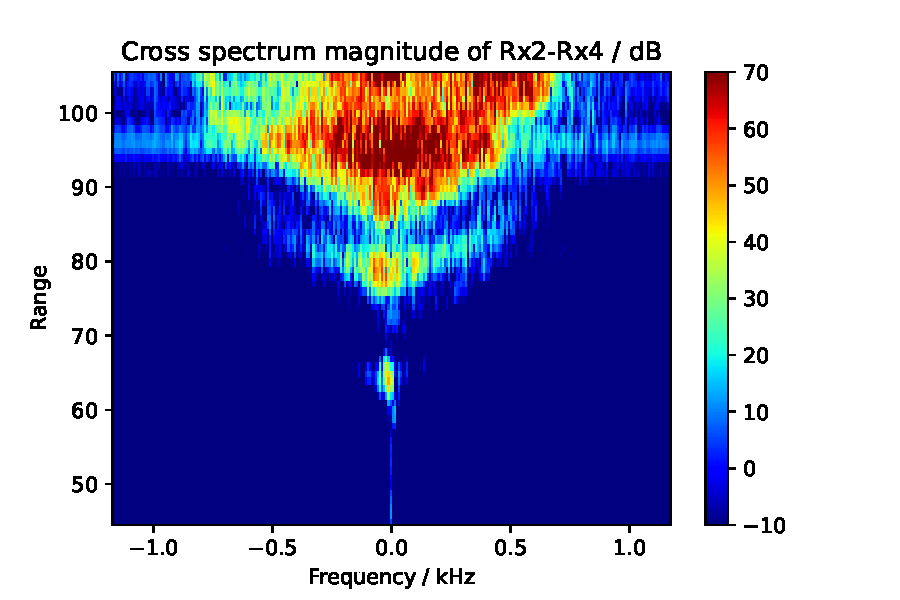
\includegraphics[width=\textwidth]{graphics/t4/t4-mag-2-4.pdf}
    \caption{Task 4: Magnitude of cross spectrum of Receivers 2 and 4.}
    \label{fig:t4-mag-2-4}
    \end{minipage}\hfill
    \begin{minipage}{0.48\textwidth}
        \centering
             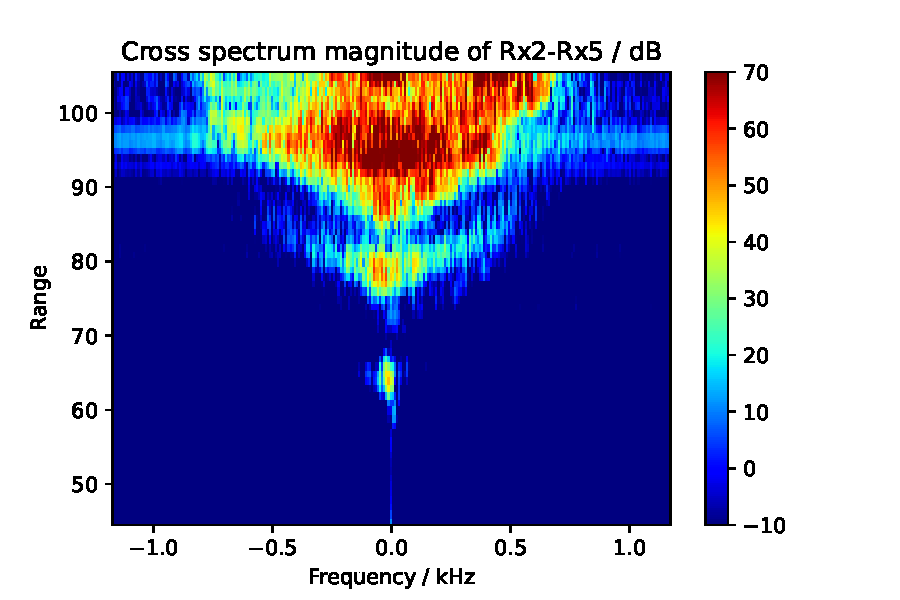
\includegraphics[width=\textwidth]{graphics/t4/t4-mag-2-5.pdf}
    \caption{Task 4: Magnitude of cross spectrum of Receivers 2 and 5.}
    \label{fig:t4-mag-2-5}
    \end{minipage}
\end{figure}

\begin{figure}[H]
    \centering
    \begin{minipage}{0.48\textwidth}
        \centering
        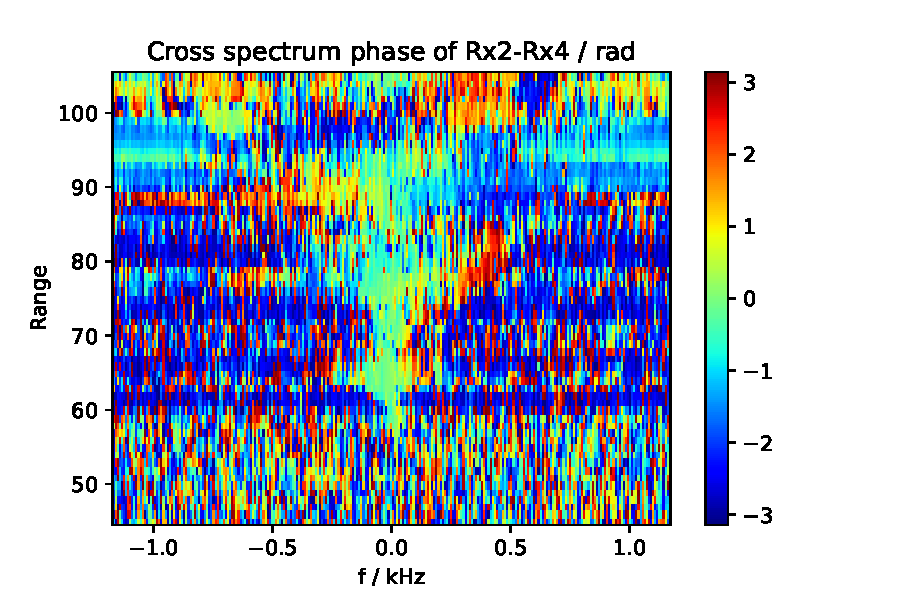
\includegraphics[width=\textwidth]{graphics/t4/t4-phase-2-4.pdf}
    \caption{Task 4: Phase of cross spectrum of Receivers 2 and 4.}
    \label{fig:t4-phase-2-4}
    \end{minipage}\hfill
    \begin{minipage}{0.48\textwidth}
        \centering
        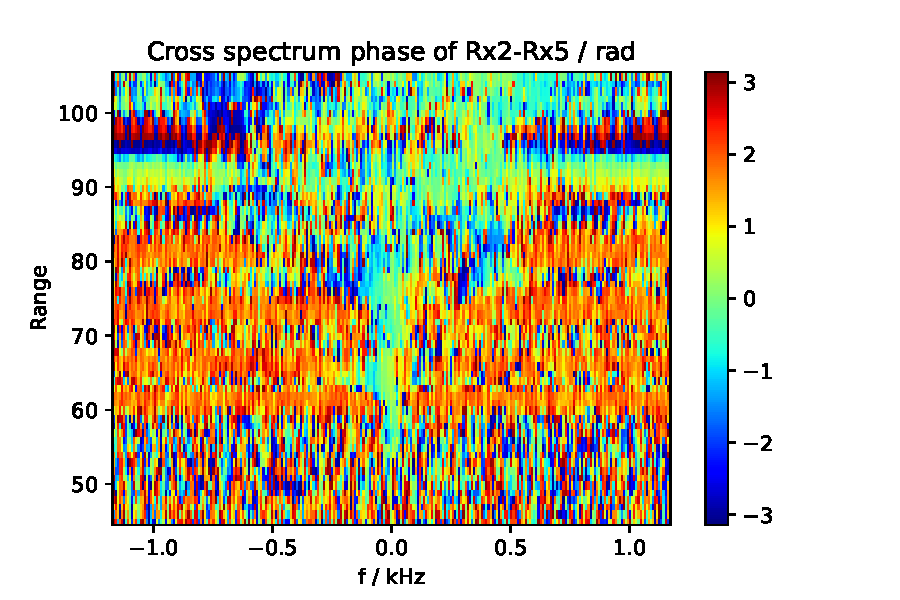
\includegraphics[width=\textwidth]{graphics/t4/t4-phase-2-5.pdf}
    \caption{Task 4: Phase of cross spectrum of Receivers 2 and 5.}
    \label{fig:t4-phase-2-5}
    \end{minipage}
\end{figure}

\begin{figure}[H]
    \centering
    \begin{minipage}{0.48\textwidth}
        \centering
        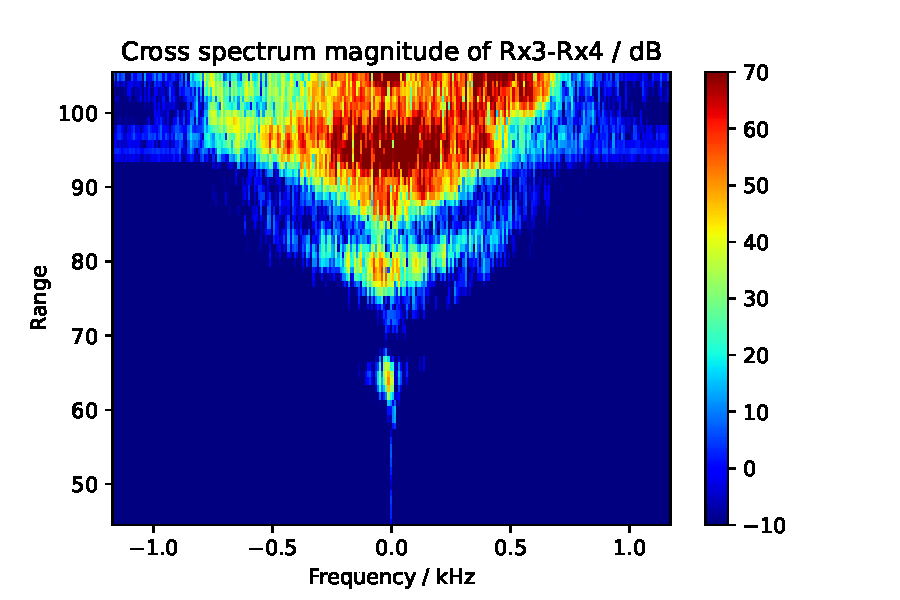
\includegraphics[width=\textwidth]{graphics/t4/t4-mag-3-4.pdf}
    \caption{Task 4: Magnitude of cross spectrum of Receivers 3 and 4.}
    \label{fig:t4-mag-3-4}
    \end{minipage}\hfill
    \begin{minipage}{0.48\textwidth}
        \centering
             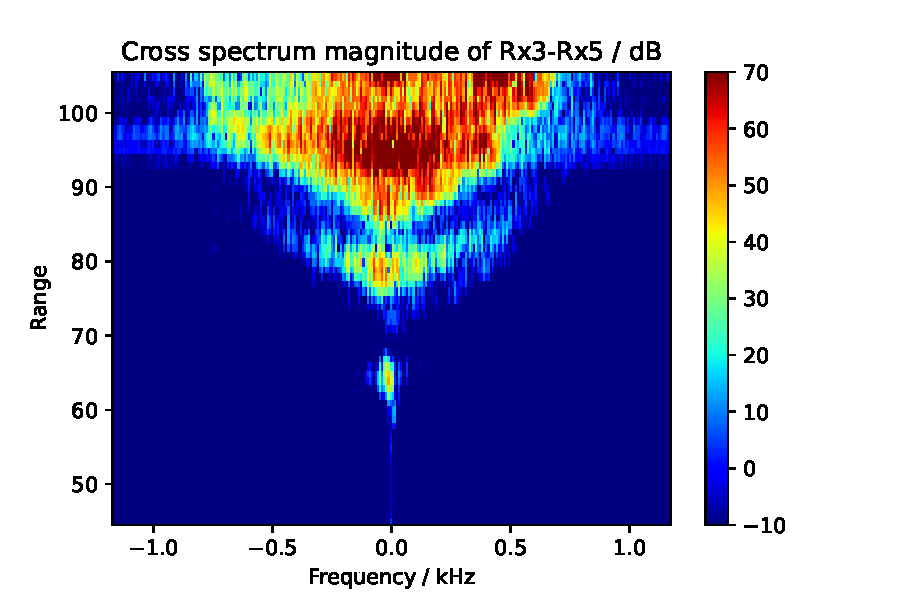
\includegraphics[width=\textwidth]{graphics/t4/t4-mag-3-5.pdf}
    \caption{Task 4: Magnitude of cross spectrum of Receivers 3 and 5.}
    \label{fig:t4-mag-3-5}
    \end{minipage}
\end{figure}

\begin{figure}[H]
    \centering
    \begin{minipage}{0.48\textwidth}
        \centering
        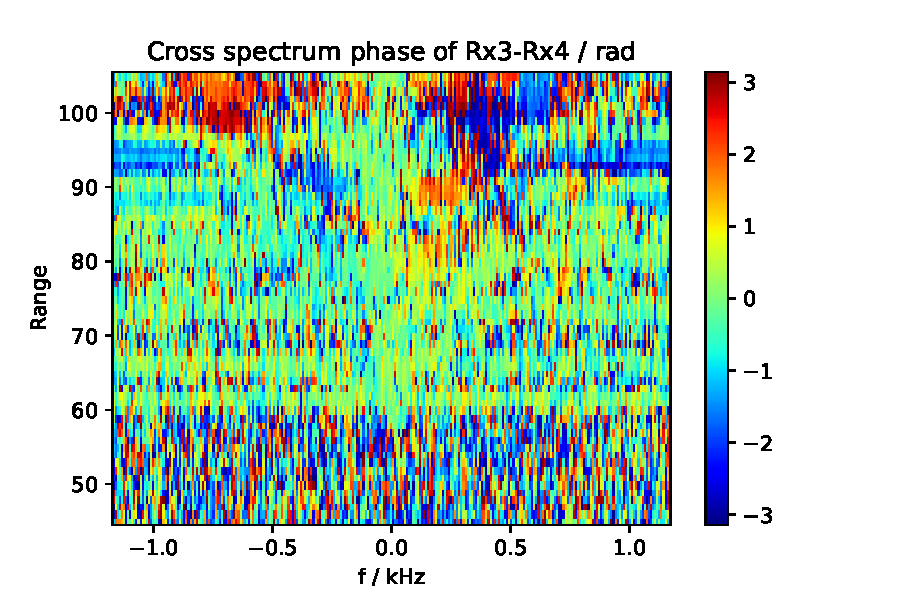
\includegraphics[width=\textwidth]{graphics/t4/t4-phase-3-4.pdf}
    \caption{Task 4: Phase of cross spectrum of Receivers 3 and 4.}
    \label{fig:t4-phase-3-4}
    \end{minipage}\hfill
    \begin{minipage}{0.48\textwidth}
        \centering
        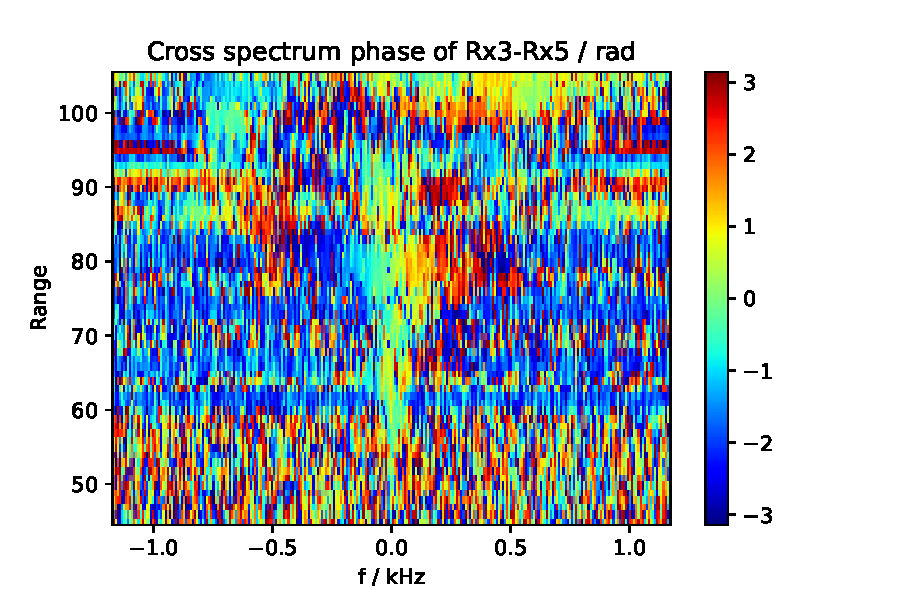
\includegraphics[width=\textwidth]{graphics/t4/t4-phase-3-5.pdf}
    \caption{Task 4: Phase of cross spectrum of Receivers 3 and 5.}
    \label{fig:t4-phase-3-5}
    \end{minipage}
\end{figure}


\end{document}
